\chapter{Non-Linear Centroidal Model Predictive Controller \label{chapter:Centroidal_mpc}}
In Chapter~\ref{chapter:simplified_benchmarking} we benchmarked several implementations of simplified model controllers. Modeling the robot with a simplified model may restrict the motion of the robot to a well-defined subset of motion primitives. For example, when the robot is described using a LIPM (see Section~\ref{sec:lip}), the CoM height must be kept constant and at least one foot must be in contact with the environment.
This chapter attempts at lowering this limitation by presenting a Non-Linear Model Predictive Controller for humanoid robot locomotion with online step adjustment capabilities. The proposed controller considers the centroidal dynamics of the system to compute the desired contact forces, torques, and contact locations. Differently from bipedal walking architectures based on simplified models, the presented approach considers the reduced centroidal model, thus allowing the robot to perform highly dynamic movements while keeping the control problem still treatable online. We show that the proposed controller can automatically adjust the contact location in both single- and double-support phases. The overall approach is then tested with a simulation of one-leg and two-leg systems performing jumping and running tasks, respectively. Finally, we validate the proposed controller in a specific version of the three-layer controller architecture of Figure~\ref{fig:three-layer}. However, differently from the original design, the simplified model controller is replaced by the \emph{Reduced model control} layer that implements the controller presented in this chapter -- see Figure~\ref{fig:centroidal_mpc_architecture}.
The overall architecture is finally tested on the position-controlled Humanoid Robot iCub v3 -- Section~\ref{sec:iCub3}. The results show that the proposed strategy prevents the robot from falling while walking and pushed with external forces up to 40 Newton for 1 second applied to the robot arm.
\par
The chapter is organized as follows. Section~\ref{sec:reduced_mpc} introduces the control problem. Section~\ref{sec:centroidal_mpc_results} presents the simulation results for different kinds of floating base systems and on the position-controlled Humanoid Robot iCub v3 -- Section~\ref{sec:iCub3}. Finally, Section~\ref{sec:centroidal_mpc_conclusion} concludes the chapter.
\par
\begin{figure}[t]
    \centering
    \includegraphics{chapter_centroidal_mpc/figures/architecture.tikz}
    \caption[Centroidal MPC embedded into a three layer controller architecture]{Centroidal MPC embedded into a three layer controller architecture.}
    \label{fig:centroidal_mpc_architecture}
\end{figure}

The content of this chapter appears in:
\fciteWithVideoAndCode{Romualdi2022OnlineAdjustment}{https://www.youtube.com/watch?v=u7vCgE2w_vY9}{https://www.youtube.com/watch?v=u7vCgE2w\_vY9}{https://github.com/ami-iit/paper_romualdi_2022_icra_centroidal-mpc-walking}{ami-iit/paper\_romualdi\_2022\_icra\_centroidal-mpc-walking}
\section{Centroidal model predictive controller}
\label{sec:reduced_mpc}
Let us assume the presence of a high-level contact planner that generates only the contact location and times, for example, the one presented in Section~\ref{sec:footsteps_trajectory}~\citep{8594277}.
The control objective of the reduced model is to implement a control law that generates feasible contact wrenches ${}_{\mathcal{C}_i[\mathcal{I}]}\mathrm{f}_i$ and locations $p_i$ while considering the centroidal dynamics of the floating base system and a nominal set of contact positions and timings. Here we denote by $\mathcal{C}_i[\mathcal{I}] = (p_i, \mathcal{I})$, the frame placed on the robot contact location $p_i$ and oriented as the inertial frame $\mathcal{I}$, where $i\in\mathbb{N}$ such that $1\le i \le n_c$, with $n_c$ is the number of admissible contacts. The control problem is formulated using the Model Predictive Control (MPC) framework. 
\par
The control objective is achieved by framing the controller as a constrained optimization problem composed of three main elements, namely: the \emph{prediction model}, an \emph{objective function}, and a set of \emph{inequality constraints}.
\par
What follows is a complete description of the task composing the optimal control problem. In mode detail, Section~\ref{sec:centroidal_mpc_dynamics} introduces the model considered in the controller as prediction. Section~\ref{sec:mpc_tasks_formulation} presents the terms that describe the control objective. Finally, in Section~\ref{sec:mpc_constraints} we discuss the inequality constraints required to guarantee a feasible walking pattern.

\subsection{Prediction model}
\label{sec:centroidal_mpc_dynamics}

Given a frame $\bar{G} = (x_\text{CoM},[\mathcal{I}])$, the centroidal momentum rate of change ${}_{\bar{G}} \dot{h}$ balances the external spatial force applied to the robot~\eqref{eq:centroidal_momentum_dynamics_mixed}:
\begin{equation}
    \label{eq:mpc_centroidal_dynamics}
    {}_{\bar{G}} \dot{{h}} = \sum_{j = 1}^{n_c} \begin{bmatrix}
	I_3 & {0}_{3\times 3} \\
	\left({p}_j - {x}_\text{CoM}\right)\times & I_3 
	\end{bmatrix} {}_{\mathcal{C}_j[\mathcal{I}]}\mathrm{f}_j + m \bar{g},
\end{equation}
where $\bar{g} = \begin{bmatrix} 0&0&-g&0&0&0 \end{bmatrix}^\top$ is the 6D gravity acceleration vector.
\par
We now recall that, given a rigid body in contact with a rigid environment and assuming that the contact surface is described by a rectangle. Then, the contact wrench acting on the rigid body is uniquely described by four pure forces acting on the corner of the contact surface~\citep{Caron2015StabilityAreas}. Indeed, in the case of a rectangular contact surface, twelve variables define the six-dimensional wrench. Thanks to this choice, several contact configurations can be modeled independently, depending on the number of points in contact~\citep{Dafarra2020Whole-BodyApproach,dai2014whole}. Given the relation between pure forces and contact wrench, we rewrite the centroidal dynamics \eqref{eq:mpc_centroidal_dynamics} as follows:
\begin{equation}
 	{}_{\bar{G}} \dot{h} = \sum_{i = 1}^{n_c} \sum_{j = 1}^{n_v} \begin{bmatrix}
       I_3 \\
       (p_{i} + R _{\mathcal{C} _ {i} } \; {}^{\mathcal{C}_i}  p_{v_{i,j}} - x_{\text{CoM}})\times
     \end{bmatrix} f_{i,j} + m\bar{g}.
     \label{eq:centroidal_dynamics}
\end{equation}
We denote by $n_v$ the number of vertices associated with the contact surface, commonly $n_v = 4$. ${}^{\mathcal{C}_i} p_{v_{i,j}}$ is the position of the vertex $j$ of the contact $i$ expressed with respect to the frame associated with the contact surface $\mathcal{C}_i$. $f_{i,j}$ is the pure force applied to the vertex $j$ of the contact $i$ expressed in the inertial frame $\mathcal{I}$.
\par
Assume a rigid body that interacts with the environment. The contact force is supposed to be non-null only if the point is in contact with the environment. The condition is called \emph{complementary condition} and writes as:
\begin{equation}
    h(p_{i})n(p_{i})^\top f_i = 0,
    \label{eq:complementary_condition}
\end{equation}
where $h$ computes the distance between the point $p_{i}$ and the environment and $n(p_{i})$ returns the normal direction to the contact surface at the point $p_{i}$. 


Since the proposed controller assumes the knowledge of the contact sequence, it is possible to define the variable $\Gamma_i \in \{0, 1\}$ for each contact. $\Gamma_i$ represents the contact state at a given instant. $\Gamma_i(t) = 0$ indicates that the contact $i$-th is not active at the time $t$, while, when $\Gamma_i(t) = 1$ the contact is active. 
Due to this assumption, it is not necessary to introduce the contact force complementary condition~\eqref{eq:complementary_condition}. In fact, considering the complementary condition in an optimization algorithm may cause problems for the nonlinear optimization solvers because the constraint Jacobian becomes singular, thus violating the linear independence constraint qualification (LICQ) on which most solvers rely -- see Section~\ref{sec:kkt_conditions}~\citep{BettsPractical2010}.
As a consequence of the introduction of $\Gamma_i$, \eqref{eq:centroidal_dynamics} is rewritten as
\begin{IEEEeqnarray}{cl}
\phantomsection     \label{eq:centroidal_dynamics_discretized} \IEEEyesnumber \IEEEyessubnumber*
    {}_{\bar{G}} \dot{h} &=\sum_{i = 1}^{n_c} \sum_{j = 1}^{n_v} \begin{bmatrix}
      I_3 \\
      (p_{i} + R _{\mathcal{C} _ {i}}\; {}^{\mathcal{C}_i}  p_{v_{i,j}}  - x_{\text{CoM}})\times
    \end{bmatrix} \Gamma_i f_{i,j} + m\bar{g}\\
    &=\mathcal{F}\left(p_{i}, x_{\text{CoM}}, f_{i,j}\right).
\end{IEEEeqnarray}
In $\mathcal{F}$, we explicitly express the dependency on the unknown variables, namely: the contact location $p_{i}$,  the CoM position $x_{\text{CoM}}$ and the contact forces $f_{i,j}$.
We finally notice that the centroidal angular momentum dynamics~\eqref{eq:centroidal_dynamics_discretized} is not convex in the variables $f_{i,j}$, $p_{i}$ $x_{\text{CoM}}$, this fact may induce to complexity in treating the centroidal dynamics as a prediction model. 
\par
Since the MPC aims to compute the control outputs online, the optimal control problem formulation should be as general as possible in the number of active contact phases in the prediction windows. For this reason, we consider each contact location as a continuous variable subject to the following dynamics:
\begin{equation}
    \dot{p} _{i}= ( 1 - \Gamma _ i)  v_{i},
    \label{eq:contact_dynamics}
\end{equation}
where we define $v _ {\mathcal{C}_i}$ as the \emph{contact velocity}\footnote{We want to warn the reader that the term \emph{contact velocity} could be misleading. Indeed, when the contact is active, its velocity is always assumed to be zero. $v_{i}$ is just an auxiliary variable that allows us to treat the contact location as a continuous variable; $v_{i}$ will be different from zero only when the contact is not active.}. To give the reader a better understanding of Equation~\eqref{eq:contact_dynamics}, we can imagine that when the contact is active, that is, $\Gamma_i = 1$, \eqref{eq:contact_dynamics} becomes $\dot{p} _{i} = 0$. In other words, the contact location is kept constant if the contact is active.

\subsection{Objective function \label{sec:mpc_tasks_formulation}}
The objective function is defined in terms of several tasks. In the following sections, we discuss the contribution of each task.

\subsubsection{Contact force regularization}

Each contact link is subject to the effect of different contact forces. Since the net effect is given by the sum of all these forces, we want them to be as similar as possible. As a consequence, we add a task that weighs the difference of each contact force from the average for a given contact link:
\begin{equation}
    \Psi_{f_{i,j}} = \frac{1}{2} \left\| \frac{1}{n_v}\sum_{w = 1}^{n_v} f_{i,w} - f_{i,j} \right\|^2_{\Lambda_{f_{i,j}}},
\end{equation}
where $\Lambda_{f_{i,j}}$ is a positive definite diagonal matrix, i.e., $\Lambda_{f_{i,j}} \succeq 0$. $f_{i,w}$ is given by the sum of all the forces acting by the environment on the link $i$ in contact as
\begin{equation}
    f_{i,w} = \sum_{w = 1}^{n_v} f_{i,j}.
\end{equation}
\par
To prevent the controller from providing solutions with a huge rate of change of the contact force, we decided to minimize the contact force derivative by considering the following task:
\begin{equation}
    \label{eq:mpc_task_dotf_initial}
    \Psi_{\dot{f}_{i,j}} = \frac{1}{2} \left\|  \dot{f}_{i,j} \right\|^2_{\Lambda_{\dot{f}_{i,j}}},
\end{equation}
where $\Lambda_{\dot{f}_{i,j}}$ is a positive defined diagonal matrix.
In our control problem, the time derivative of the contact force $\dot{f}_{i,j}$ is not considered as an optimization variable. To overcome this limitation, we decided to replace $\dot{f}_{i,j}$ with its first-order numerical approximation:
\begin{equation}
    \label{eq:mpc_numerical_approximation_df}
    \dot{f}_{i,j} = \frac{f_{i,j}[k] - {f}_{i,j}[k-1]  }{\diff t}.
\end{equation}
Here, $\diff t$ is the controller sampling rate. $f_{i,j}[k]$ ${f}_{i,j}[k-1]$ represent, respectively, the contact force at the time instant $t_0 + k \diff t$ and $t_0 + (k-1) \diff t$.
Substituting~\eqref{eq:mpc_numerical_approximation_df} into the task~\eqref{eq:mpc_task_dotf_initial}, we obtain the final formulation of the contact force rate-of-change regularization task.
\begin{equation}
    \label{eq:mpc_task_dotf}
    \Psi_{\dot{f}_{i,j}} = \frac{1}{2} \norm{\frac{f_{i,j}[k] - {f}_{i,j}[k-1]  }{\diff t}}^2_{\Lambda_{\dot{f}_{i,j}}}.
\end{equation}

\subsubsection{Centroidal momentum tracking task}
To follow a desired centroidal momentum trajectory, we minimize the weighted norm of the error between the robot's centroidal quantities and the desired nominal trajectory:
\begin{equation}
    \Psi_{h} = \frac{1}{2} \left\| \prescript{}{\bar{G}}{h}^{\omega ^n} - \prescript{}{\bar{G}}{h}^\omega \right\|^2_{\Lambda_{h}} + \frac{1}{2} \left\| x_{\text{CoM}} ^ n -x_{\text{CoM}}  \right\|^2_{\Lambda_{\text{CoM}}}, 
    \label{eq:task_centroidal}
\end{equation}
where $\Lambda_h$ and $\Lambda_{\text{CoM}}$ are two positive definite diagonal matrices. The desired angular momentum $\prescript{}{\bar{G}}{h}^{\omega ^n}$ and CoM position $x_{\text{CoM}} ^ n$, should be considered as regularization terms. As a consequence, their purpose is to \emph{drive} the optimal control problem to the desired feasible solution. In other words, $\prescript{}{\bar{G}}{h}^{\omega ^n}$ and $x_{\text{CoM}} ^ n$ could not be a dynamically consistent trajectory. In our specific scenario we consider $\prescript{}{\bar{G}}{h}^{\omega ^n}$ always equal to zero, while $ x_{\text{CoM}} ^ n$ is a fifth-order spline passing through the nominal contact locations, whose initial and final velocity and acceleration are zero. 

\subsubsection{Contact location regularization}
To reduce the difference between the nominal contact location and the one computed by the controller, we consider the following regularization task:
\begin{equation}
    \Psi_{p_{i}} = \frac{1}{2} \left\| p_{i}^n  - p_{i}  \right\|^2_{\Lambda_{p_{i}}}.
    \label{eq:task_contact}
\end{equation}
Here $p_{\mathcal{C}_i^n}$ is the nominal contact position provided by a high-level planner, and $\Lambda_{p_{i}}$ is a positive definite diagonal matrix.


\subsection{Inequality constraints\label{sec:mpc_constraints}}
This section contains the two sets of inequality constraints considered in the optimal control problem. 

\subsubsection{Contact force feasibility}
Similar to what we discuss for the whole-body controllers~\ref{sec:tsid_tasks} and \ref{sec:tsid_compliant_tasks}, to guarantee a \emph{weakly stable contact}~\citep{Caron2015StabilityAreas}, the contact force should belong to a second-order cone~\eqref{eq:friction_cone}. However, to simplify the friction constraint, the friction cone is often approximated by the conic combination of $n$ vectors -- Section~\ref{sec:convex_set_example}. The half-space representation of the friction cone approximation is given by a set of linear inequalities of the form 
\begin{equation}
A \; {}^{\mathcal{C} _ {i} } R _{\mathcal{C} _ {i}[\mathcal{I}]} \; f _ {i, j} \preceq b.
\end{equation}
Here $A$ and $b$ are constants and depend only on the static friction coefficient. 
\begin{figure}[t]
    \centering
    \includegraphics{chapter_centroidal_mpc/figures/contact_adjustment.tikz}
    \caption{The contact feasibility region.}
    \label{fig:contact_adjustment}
\end{figure}

\subsubsection{Contact location constraint}
The proposed controller aims to compute the contact location. In particular, the new contact position should belong to the feasibility region described by a rectangle containing the nominal contact location -- Figure~\ref{fig:contact_adjustment}.

We introduce the contact location constraint as 
\begin{equation}
    l_b\preceq {}^{\mathcal{C} _ {i} }  R_{\mathcal{I}}   (p_{i}^n - p_{i}) \preceq u_b,
\end{equation}
where $l_b$ and $u_b$ are the lower and upper bounds of the rectangle represented in the frame attached to the contact $\mathcal{C} _ {i} $.

\subsection{MPC formulation}
\label{sec:mpc_formulation}
Combining the set of tasks presented in Section~\ref{sec:mpc_tasks_formulation}, with the prediction models of Section~\ref{sec:centroidal_mpc_dynamics} and the inequality constraints described in Section~\ref{sec:mpc_constraints}), we formulate the MPC as an optimization problem. 
\par
The MPC problem is solved using a Direct Multiple Shooting method \citep{BettsPractical2010} -- Section~\ref{sec:shooting_methods}. We discretize the centroidal dynamics~\eqref{eq:centroidal_dynamics_discretized} and the contact location dynamics~\eqref{eq:contact_dynamics} by applying the Forward Euler technique with a constant sampling time $\diff t$ -- Equation~\eqref{eq:forward_euler}. The controller outputs are generated using the Receding Horizon Principle \citep{Mayne90MPC}, adopting a fixed prediction window with a length equal to $N$ samples -- Section~\ref{sec:mpc}.

The MPC formulation is finally obtained by solving the following optimization problem:
\begin{IEEEeqnarray}{CL}
\phantomsection \label{eq:mpc_centroidal_contact_optimization} \IEEEyesnumber \IEEEyessubnumber*
	\minimize_{\substack{\mathcal{X}_k, \mathcal{U}_k, \\ k = [0, N]}}& \sum_{k = 0} ^ N \left(\sum_{i,j} \Psi_{f_{i,j}} + \sum_{i, j} \Psi_{\dot{f}_{i,j}} + \Psi_h + \sum_i \Psi_{p_{i}}\right)
 \label{costFunction}\\
	\text{subject to } & {}_{\bar{G}} h[k + 1] = \mathcal{F}\left(p_{i}, x_{\text{CoM}}, f_{i,j}\right) \diff t + {}_{\bar{G}} h[k] \label{eq:mpc_centroidal_centroidal_dynamics_optimization} \\
	& x_{\text{CoM}}[k+1] = \frac{{}_{\bar{G}} h^p[k]}{m} \diff t  + x_{\text{CoM}}[k] \\
	& p_{i}[k + 1] = p_{i}[k] + ( 1 - \Gamma _ i[k]) v_{i}[k] \diff t \label{eq:mpc_centroidal_contact_dynamics_optimization}\\
	& A \; {}^{\mathcal{C} _ {i} } R _{\mathcal{C} _ {i}[\mathcal{I}]} \; f _ {i, j} \preceq b.
 \label{eq:mpc_centroidal_contact_feasibility_optimization}\\ 
	&        l_b\preceq {}^{\mathcal{C} _ {i} }  R_{\mathcal{I}}   (p_{i}^n - p_{i}) \preceq u_b \label{eq:mpc_centroidal_contact_position_optimization}.
\end{IEEEeqnarray}
Where the contact dynamics constraint~\eqref{eq:mpc_centroidal_contact_dynamics_optimization}, the contact force feasibility~\eqref{eq:mpc_centroidal_contact_feasibility_optimization} and the contact position constraint~\eqref{eq:mpc_centroidal_contact_position_optimization} are repeated for each admissible contact. $\mathcal{X}_k$ and $\mathcal{U}_k$ contain, respectively, the controller state and output at a time instant $k$:
\begin{IEEEeqnarray}{c}
\phantomsection \IEEEyesnumber \IEEEyessubnumber*
    \mathcal{X}_k ^\top = \begin{bmatrix} x_{\text{CoM}}[k]^\top & \prescript{}{\bar{G}}{h}[k]^\top &  p_{i}[k]^\top \end{bmatrix}, \\
    \mathcal{U}_k ^\top = \begin{bmatrix} f_{i,j}[k]^\top &  v_{i}[k]^\top \end{bmatrix}.
\end{IEEEeqnarray}
\par
At every time step $\diff t$, we solve the optimization problem~\eqref{eq:mpc_centroidal_contact_optimization},  then we apply the control output $\mathcal{U}_0$ only, discarding all the other control inputs. The time horizon is shifted to an amount equal to $\diff t$ and the optimal control problem~\eqref{eq:mpc_centroidal_contact_optimization} is solved again with different initial conditions.
\par
Since the centroidal dynamics \eqref{eq:centroidal_dynamics} is a nonlinear non-convex function, the optimizer may find a local minimum. This may
result in a suboptimal solution for the given task. As a consequence, the initialization of the solver may play a crucial role to drive the optimizer to the desired solution.
In our case, the CoM is initialized with the nominal CoM trajectory $x_{\text{CoM}}^n$, while all other variables are set to zero.


























    











\begin{figure}[t]
        \begin{subfigure}[b]{0.32\textwidth}
        \centering
        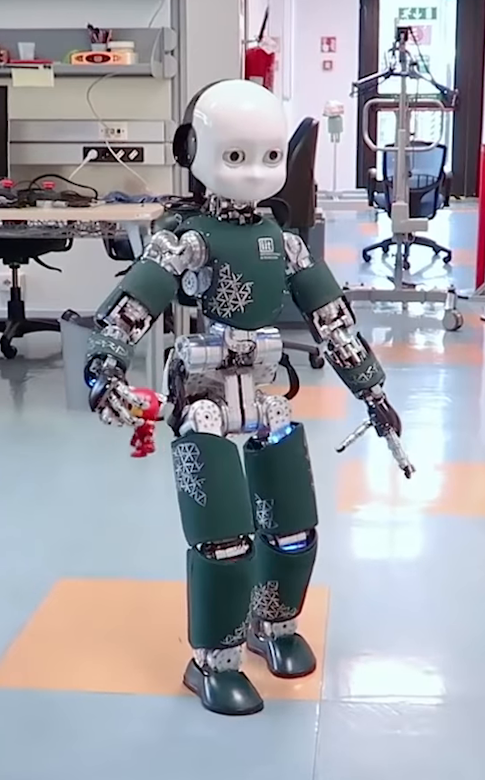
\includegraphics[width=\columnwidth]{chapter_simplified_benchmarking/figures/step1.png}
    \end{subfigure}
    \hfill
           \begin{subfigure}[b]{0.32\textwidth}
        \centering
        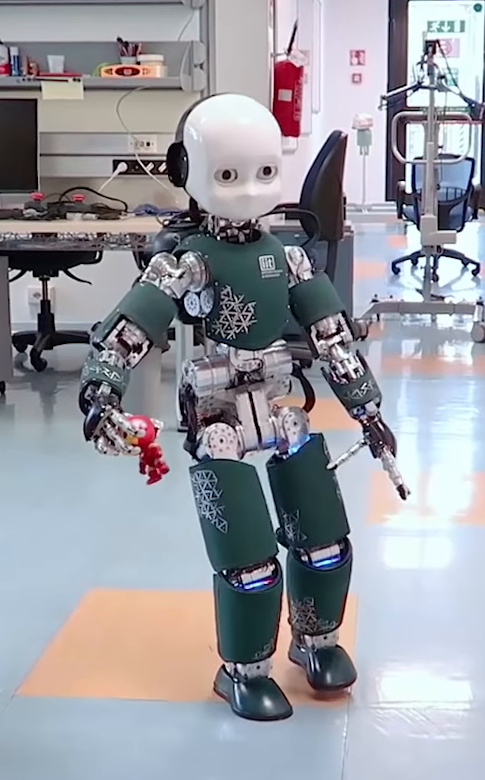
\includegraphics[width=\columnwidth]{chapter_simplified_benchmarking/figures/step2.png}
    \end{subfigure}
    \hfill
           \begin{subfigure}[b]{0.32\textwidth}
        \centering
        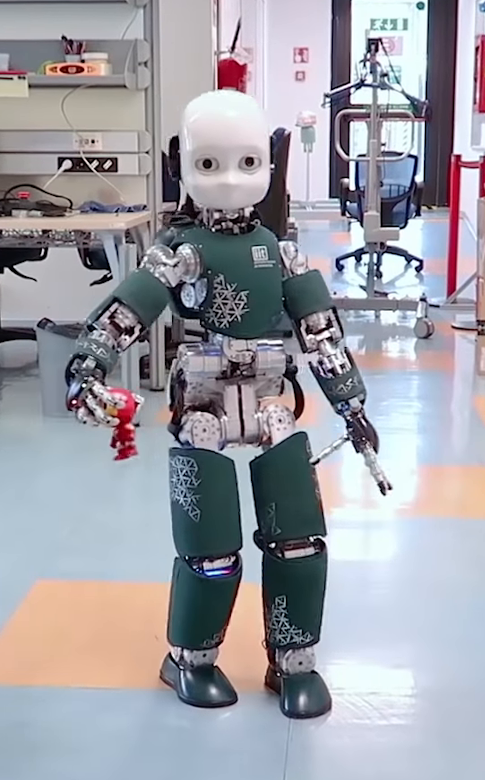
\includegraphics[width=\columnwidth]{chapter_simplified_benchmarking/figures/step3.png}
    \end{subfigure}
    \caption{The iCub robot walks with the 3 layer controller architecture of Figure~\ref{fig:three-layer-simplified-benchmarking}.}
    \label{fig:icub_walking_simplified}
\end{figure}

\section{Results}
\label{sec:results_simplified_benchmarking}
In this section, we present experiments obtained with several implementations of the simplified model controllers, namely: the \emph{instantaneous} and the \emph{predictive} controllers.

To benchmark the different simplified model controllers, we test the algorithms on the iCub humanoid robot v2.7 -- Section~\ref{sec:icub2.7}. We attach the simplified control layer to the three-layer controller architecture shown in Figure~\ref{fig:three-layer}. In this framework, the whole-body control layer implements the kinematics-based whole-body QP presented in section~\ref{sec:ik_qp}. Figure~\ref{fig:icub_walking_simplified} shows the humanoid robot iCub walking with the simplified models controller presented in this chapter.

The control architecture runs on the iCub head's computer, namely a 4-th generation Intel \textsuperscript{\tiny\textregistered} Core i7 @ $\SI{1.7}{\giga \hertz}$. In any of its implementations, the architecture takes (on average) less than $\SI{3}{\milli \second}$ to evaluate its output. The code is open source completely developed in C++: \href{https://github.com/robotology/walking-controllers}{\texttt{https://github.com/robotology/walking-controllers}}. The MPC problem presented in Section~\ref{predictive-control} is solved using the OSQP~\citep{Stellato2018} library~\footnote{Since our code is  written in pure C++, the QP problem is written by means of \texttt{osqp-eigen} a C++ wrapper for OSQP \href{https://github.com/robotology/osqp-eigen}{\texttt{https://github.com/robotology/osqp-eigen}}}.


Table~\ref{tab:max_velocity} summarizes the maximum velocities achieved using the different implementations of the control architecture. In particular, the labels \emph{instantaneous} and \emph{predictive} mean that the associated layer generates its output considering inputs and references either at the single time $t$ or for a time window, respectively. The labels, \emph{velocity} and \emph{position} control, instead, mean that the layer outputs are either desired joint velocities or position, respectively -- see Section~\ref{subsubsec-pos-vel-control}. 

\begin{table}[b]
    \centering
    \caption{Maximum forward straight walking velocities achieved using different implementations of the control architecture.
    }
    \begin{tabular}{cc|c}
         \begin{tabular}{@{}c@{}}Simplified Model  Control\end{tabular} &
         \begin{tabular}{@{}c@{}}Whole-Body QP Control\end{tabular} &
         \begin{tabular}{@{}c@{}}Max Straight Velocity (m/s)\end{tabular}\\
        \hline
        Predictive  & Velocity  &  0.1563\\
        Predictive  & Position  & 0.1645\\
        Instantaneous  & Velocity  &  0.1809\\
        Instantaneous  & Position  & 0.3372
    \end{tabular}
    \label{tab:max_velocity}
\end{table}

Let us remark that all the implemented control architectures exploit the controller presented in Section~\ref{ZMP-CoM-Controller} to attempt the stabilization of the desired center of pressure and desired center of mass position and velocity. The performance of this controller is highly dependent on the gains $K_{zmp}$ and $K_{com}$. In particular, we observed that the gains in achieving good tracking during standing and walking were not the same. For this reason, we implemented a gain-scheduling technique depending on whether the robot is walking or standing. The transition between the two sets of gains is smoothed with a minimum jerk trajectory \citep{Pattacini2010}.


To compare the simplified models controllers, we decided to perform two main experiments. These two experiments represent the maximum robot velocity that has been achieved with all architectures and the maximum velocity achieved with a specific architecture only -- see Table~\ref{tab:max_velocity}. That is, 
\begin{itemize}
    \item[-] \textbf{Experiment 1}: a forward robot speed of $\SI{0.1563}{\meter \per \second}$;
    \item[-] \textbf{Experiment 2}: a forward robot speed of $\SI{0.3372}{\meter \per \second}$.
\end{itemize}

\begin{figure}[t]
    \centering
    \begin{myframe}{Instantaneous + Position Control}
        \centering
    \begin{subfigure}[b]{0.49\textwidth}
        \centering
        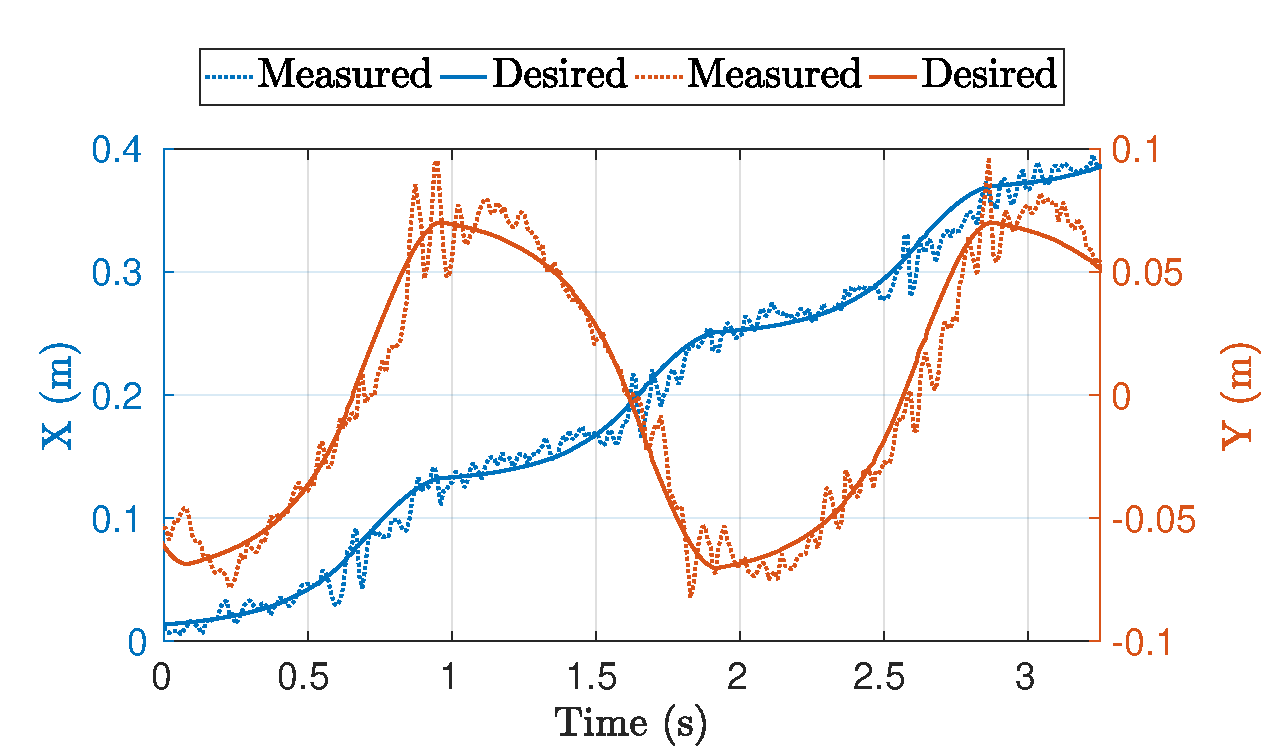
\includegraphics[width=\textwidth]{chapter_simplified_benchmarking/figures/inst_pos-min_vel-dcm.pdf}
        \caption{DCM}
        \label{fig:inst_pos-min_vel-dcm}
    \end{subfigure}
    \hfill
    \begin{subfigure}[b]{0.49\textwidth}
        \centering
        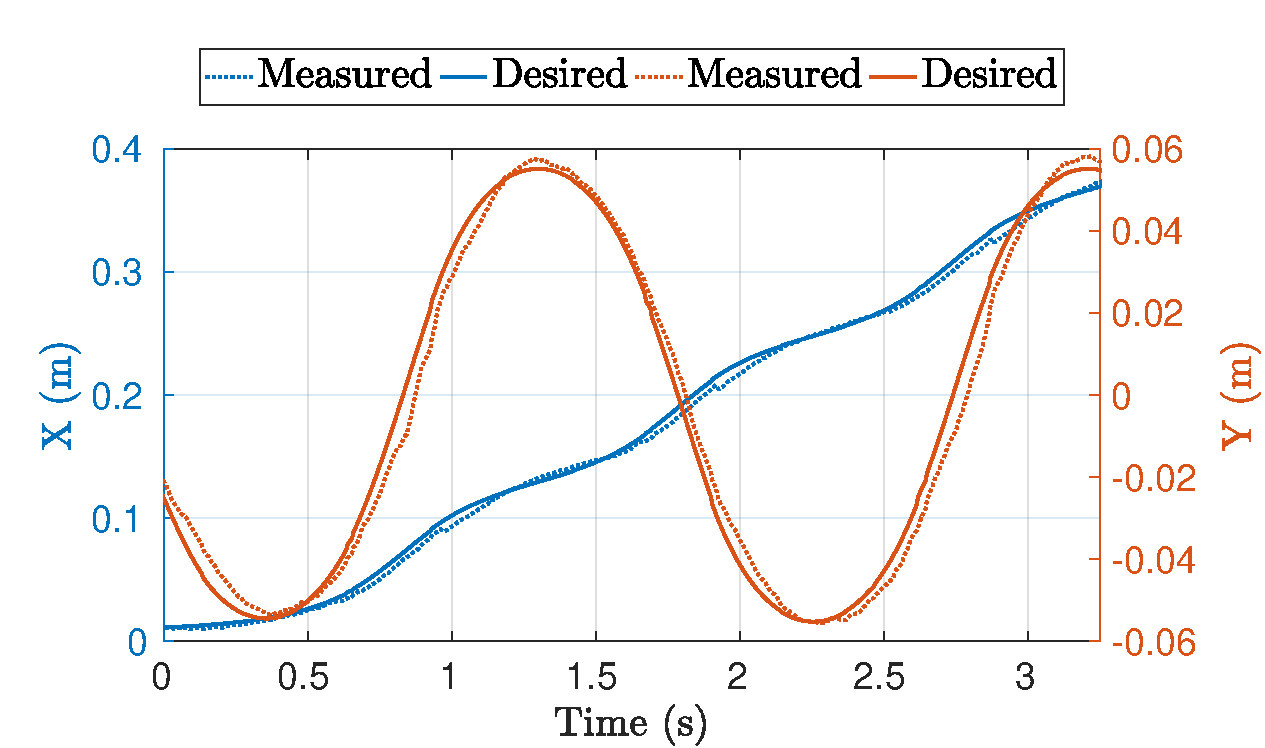
\includegraphics[width=\textwidth]{chapter_simplified_benchmarking/figures/inst_pos-min_vel-com.pdf}
        \caption{CoM}
        \label{fig:inst_pos-min_vel-com}
    \end{subfigure}
    \hfill
    \begin{subfigure}[b]{0.49\textwidth}
        \centering
        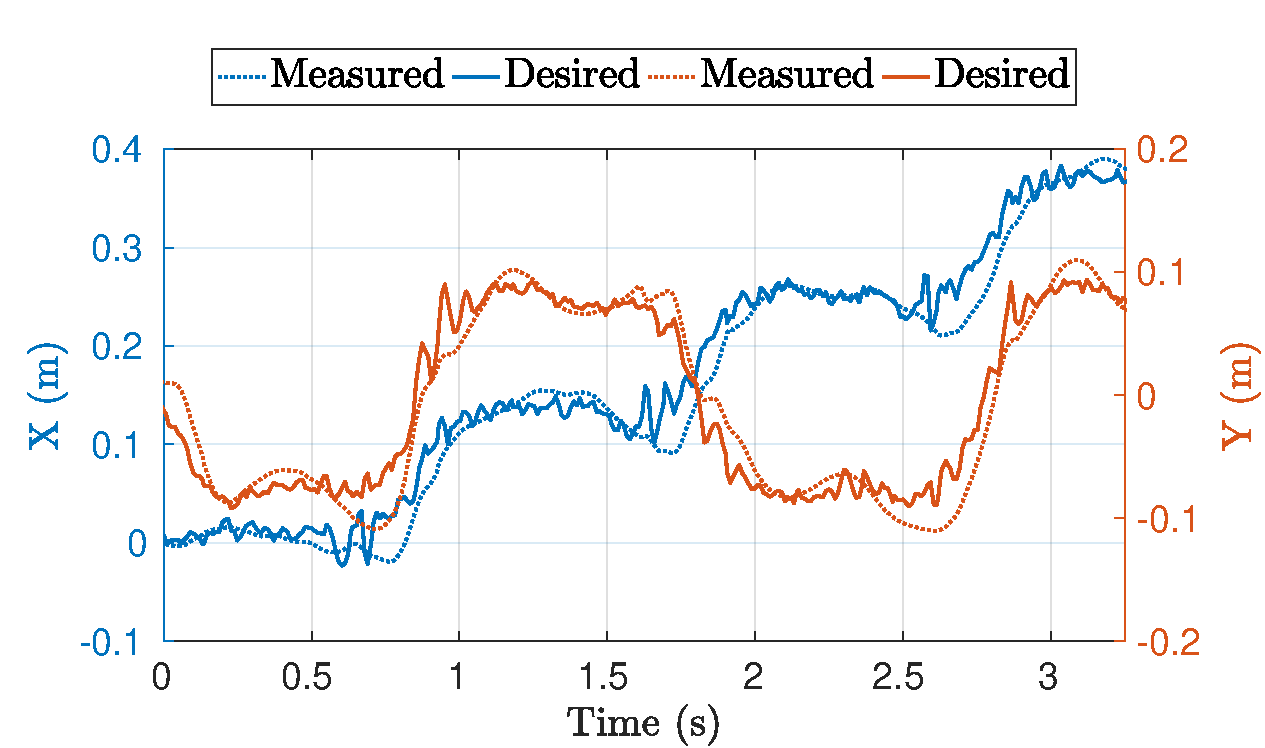
\includegraphics[width=\textwidth]{chapter_simplified_benchmarking/figures/inst_pos-min_vel-zmp.pdf}
        \caption{ZMP}
        \label{fig:inst_pos-min_vel-zmp}
    \end{subfigure}
    \end{myframe}
    \caption{Tracking of the DCM (a), CoM (b) and ZMP (c) using the instantaneous controller with the whole-body controller as position control. Walking velocity:  $\SI{0.19}{\meter \per \second}$.}
\end{figure}

\begin{figure}[t]
    \begin{myframe}{Predictive + Position Control}
     \centering
    \begin{subfigure}[b]{0.49\textwidth}
        \centering
        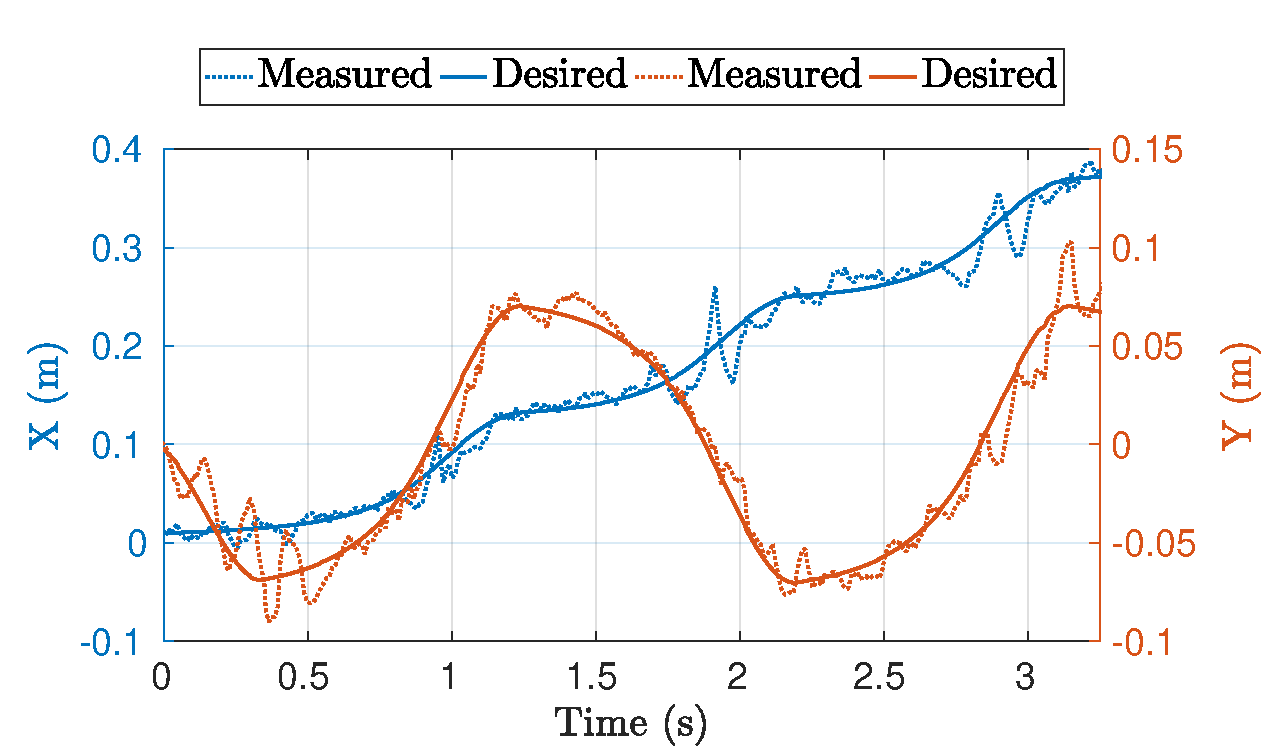
\includegraphics[width=\textwidth]{chapter_simplified_benchmarking/figures/mpc_pos-min_vel-dcm.pdf}
        \caption{DCM}
        \label{fig:mpc_pos-min_vel-dcm}
    \end{subfigure}
    \hfill
    \begin{subfigure}[b]{0.49\textwidth}
        \centering
        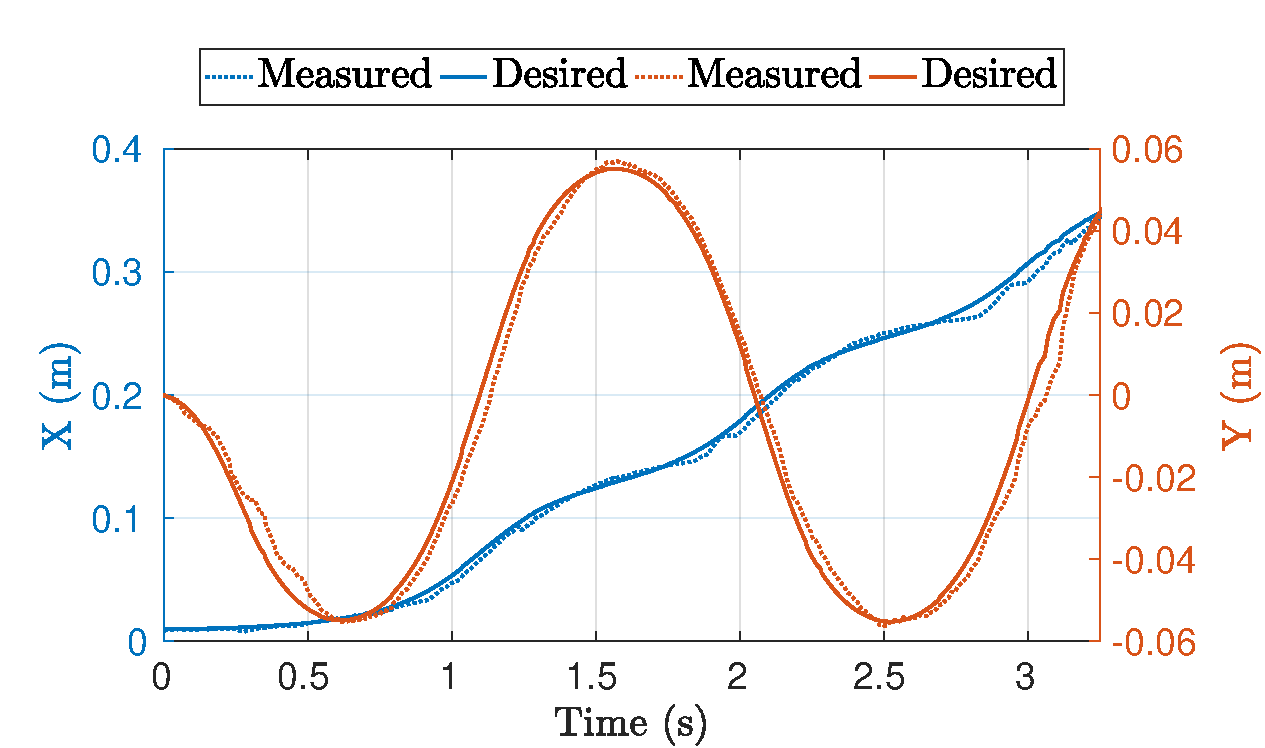
\includegraphics[width=\textwidth]{chapter_simplified_benchmarking/figures/mpc_pos-min_vel-com.pdf}
        \caption{CoM}
        \label{fig:mpc_pos-min_vel-com}
    \end{subfigure}
         \begin{subfigure}[b]{0.49\textwidth}
        \centering
        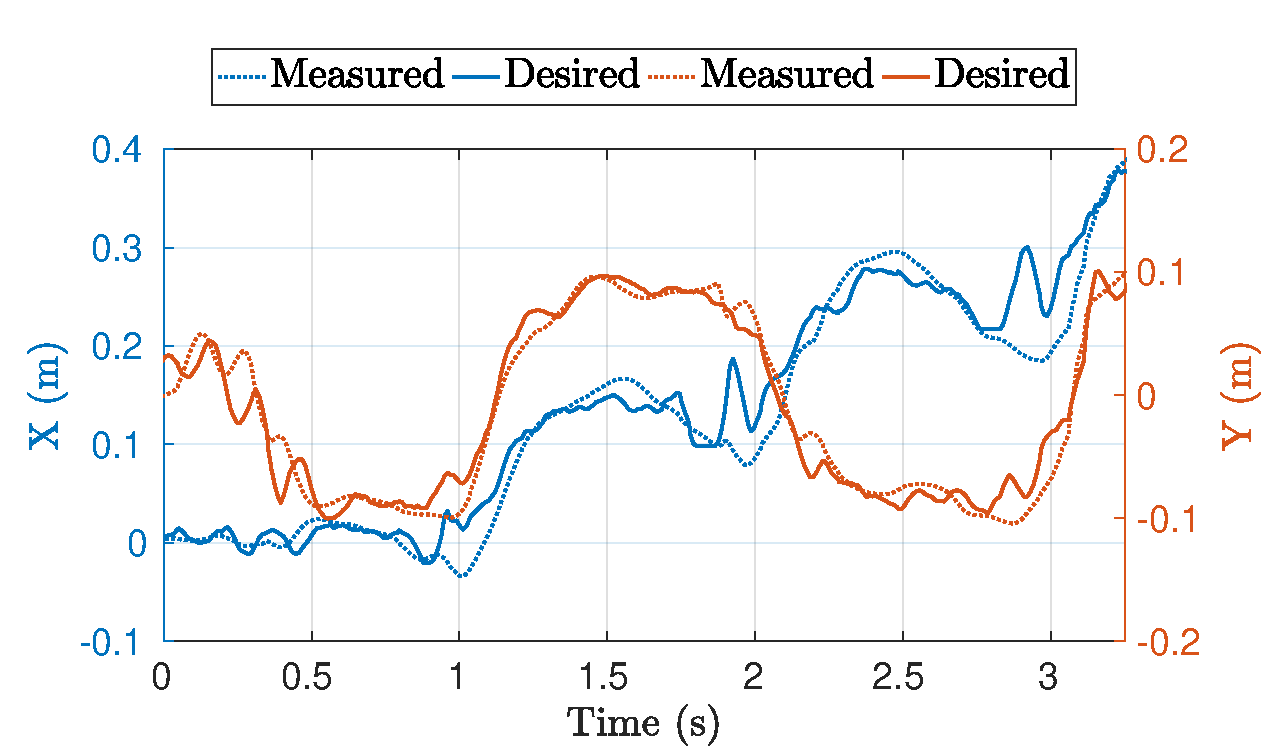
\includegraphics[width=\textwidth]{chapter_simplified_benchmarking/figures/mpc_pos-min_vel-zmp.pdf}
        \caption{ZMP}
        \label{fig:mpc_pos-min_vel-zmp}
    \end{subfigure}
    \end{myframe}
    \caption{Tracking of the  DCM (a), CoM (b) and ZMP (c) using the MPC and the whole-body controller as position control. Walking velocity:  $\SI{0.19}{\meter \per \second}$.}
\end{figure}
\begin{figure}[t]
     \vspace*{-0.1cm}
    \begin{myframe}{Instantaneous + Position Control}
    \centering
        \begin{subfigure}[b]{0.49\textwidth}
        \centering
        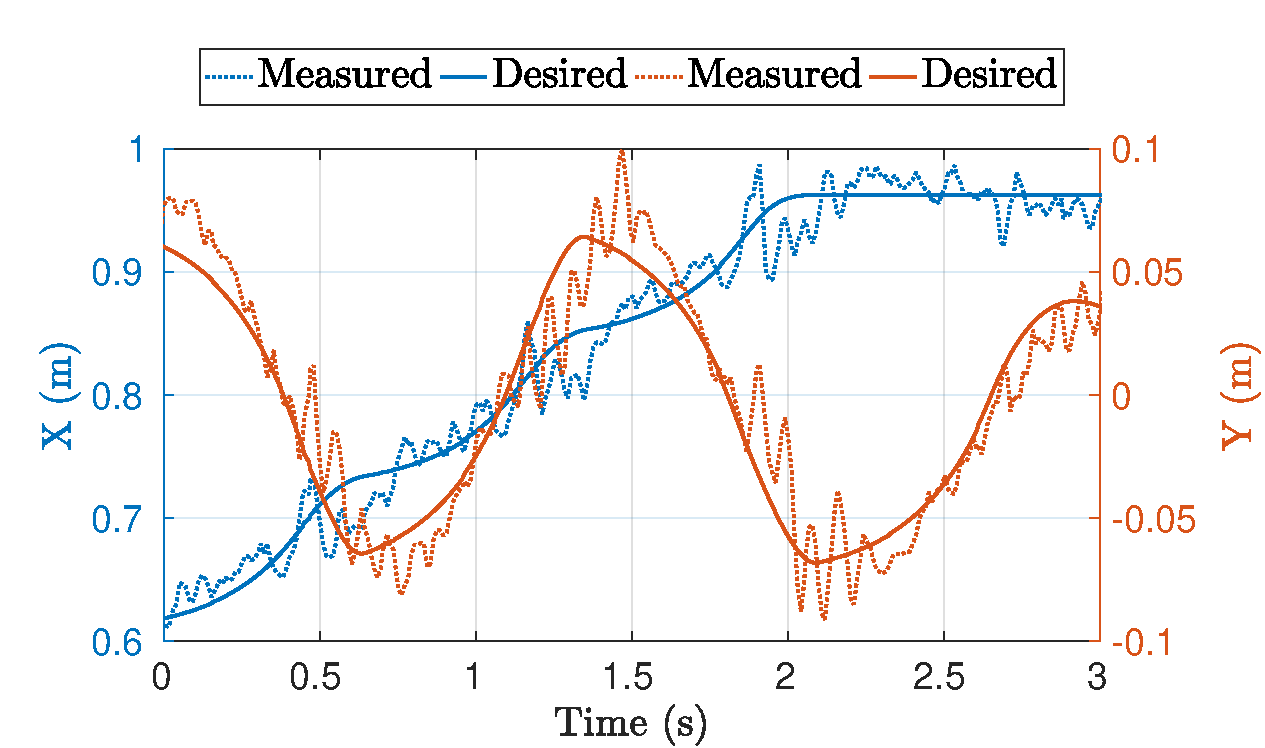
\includegraphics[width=\textwidth]{chapter_simplified_benchmarking/figures/inst_pos-max_vel-dcm.pdf}
        \caption{DCM}
        \label{fig:inst_pos-max_vel-dcm}
    \end{subfigure}
    \hfill
     \begin{subfigure}[b]{0.49\textwidth}
        \centering
        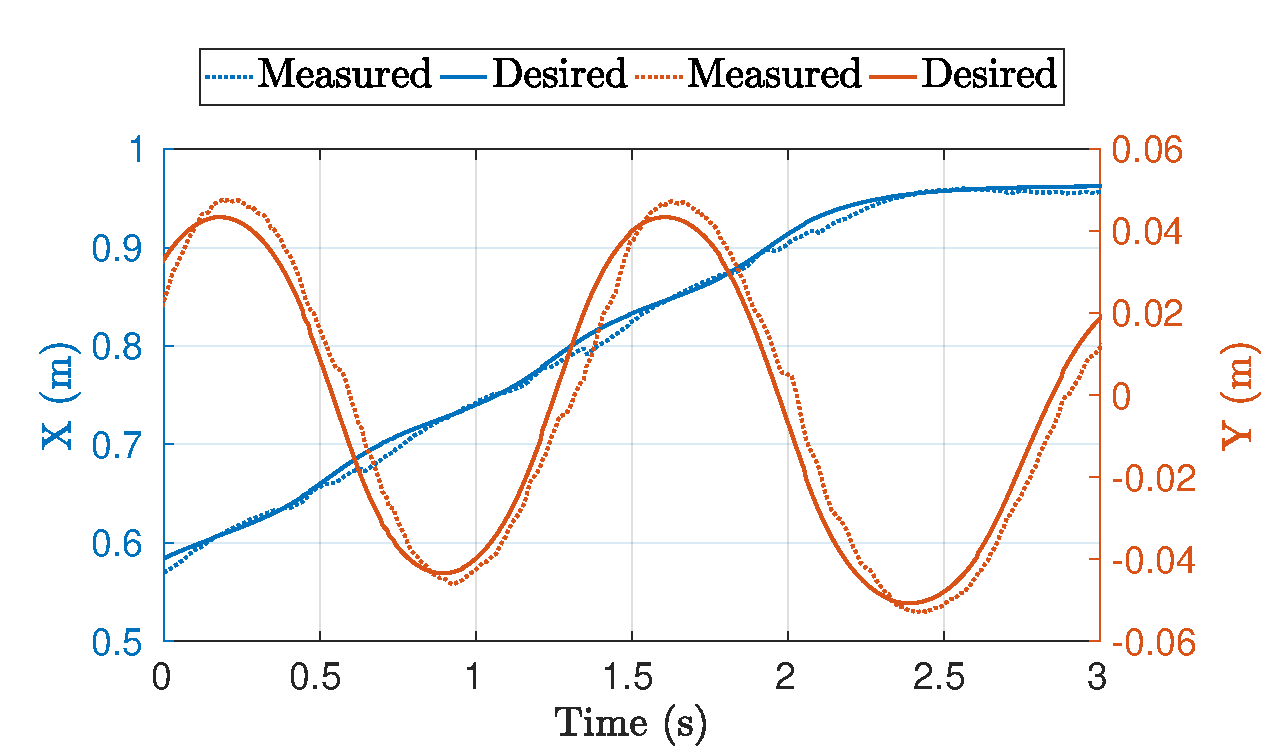
\includegraphics[width=\textwidth]{chapter_simplified_benchmarking/figures/inst_pos-max_vel-com.pdf}
        \caption{CoM}
        \label{fig:inst_pos-max_vel-com}
    \end{subfigure}
    \hfill
    \begin{subfigure}[b]{0.49\textwidth}
        \centering
        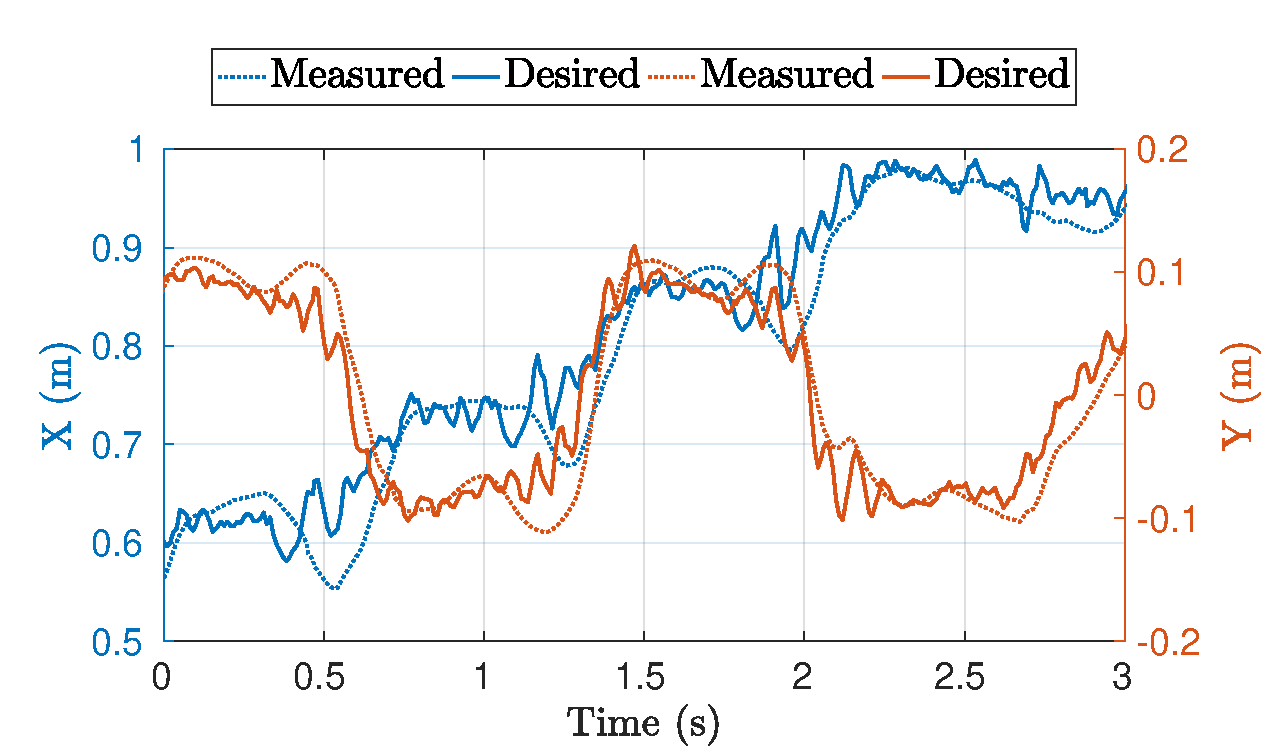
\includegraphics[width=\textwidth]{chapter_simplified_benchmarking/figures/inst_pos-max_vel-zmp.pdf}
        \caption{ZMP}
        \label{fig:inst_pos-max_vel-zmp}
    \end{subfigure}
    \end{myframe}
    \caption{Tracking of the DCM (a), CoM (b) and ZMP (c) with the instantaneous and whole-body QP control as position.  Walking velocity: $\SI{0.41}{\meter \per \second}$.}
\end{figure}
\begin{figure}[t]
    \begin{myframe}{Predictive + Position Control}
    \centering
    \begin{subfigure}[b]{0.49\textwidth}
        \centering
        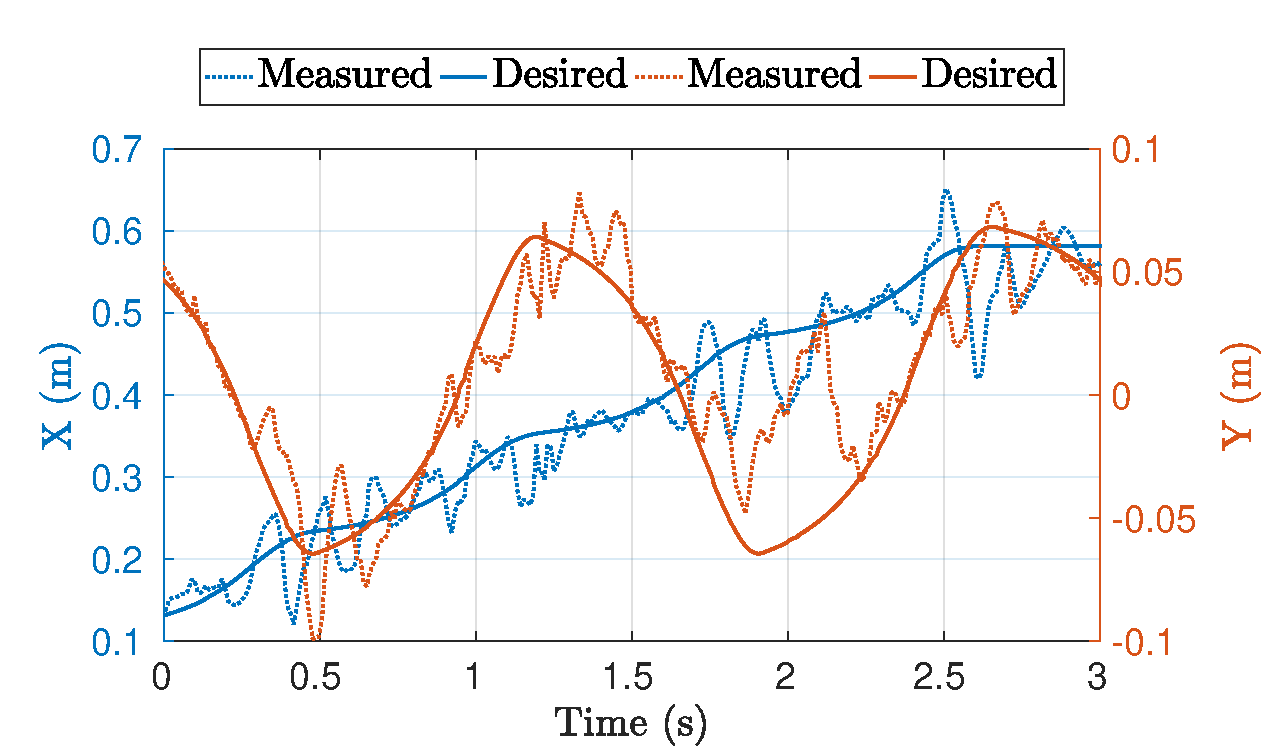
\includegraphics[width=\textwidth]{chapter_simplified_benchmarking/figures/mpc_pos-max_vel-dcm.pdf}
        \caption{DCM}
        \label{fig:mpc_pos-max_vel-dcm}
    \end{subfigure}
    \hfill
     \begin{subfigure}[b]{0.49\textwidth}
        \centering
        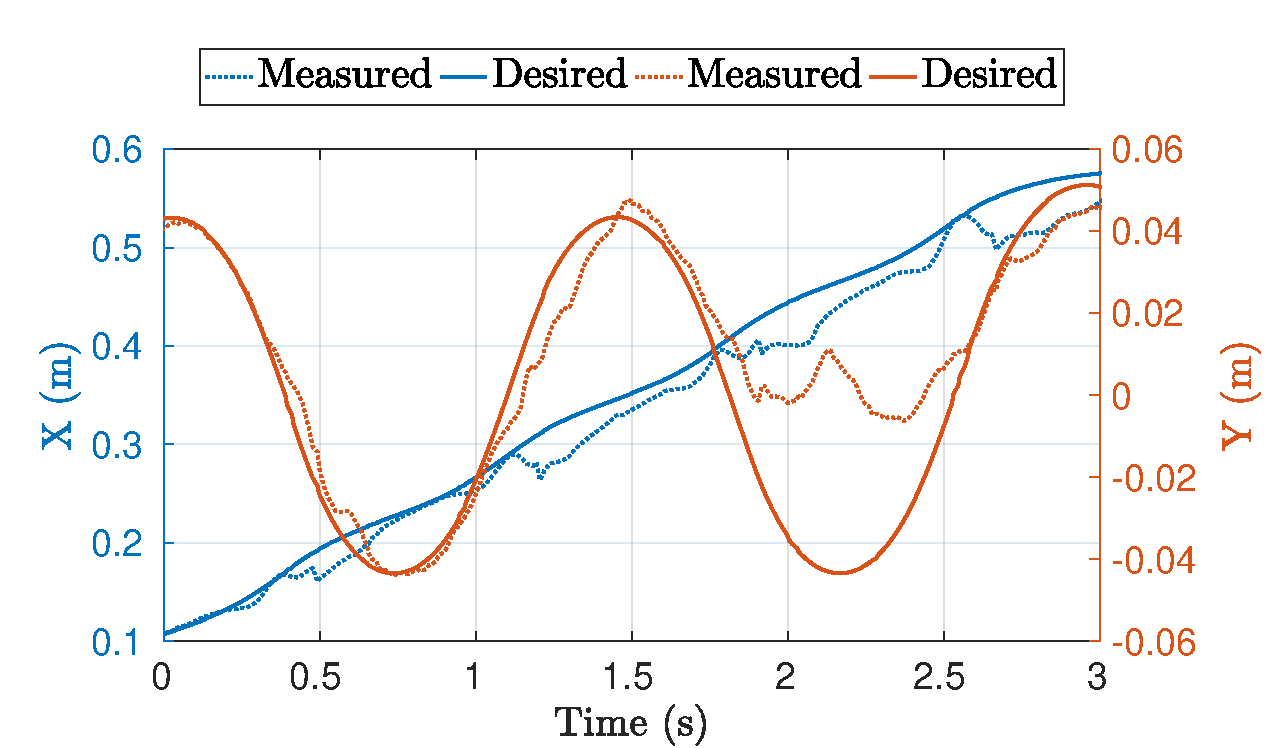
\includegraphics[width=\textwidth]{chapter_simplified_benchmarking/figures/mpc_pos-max_vel-com.pdf}
        \caption{CoM}
        \label{fig:mpc_pos-max_vel-com}
    \end{subfigure}
    \hfill
    \begin{subfigure}[b]{0.49\textwidth}
        \centering
        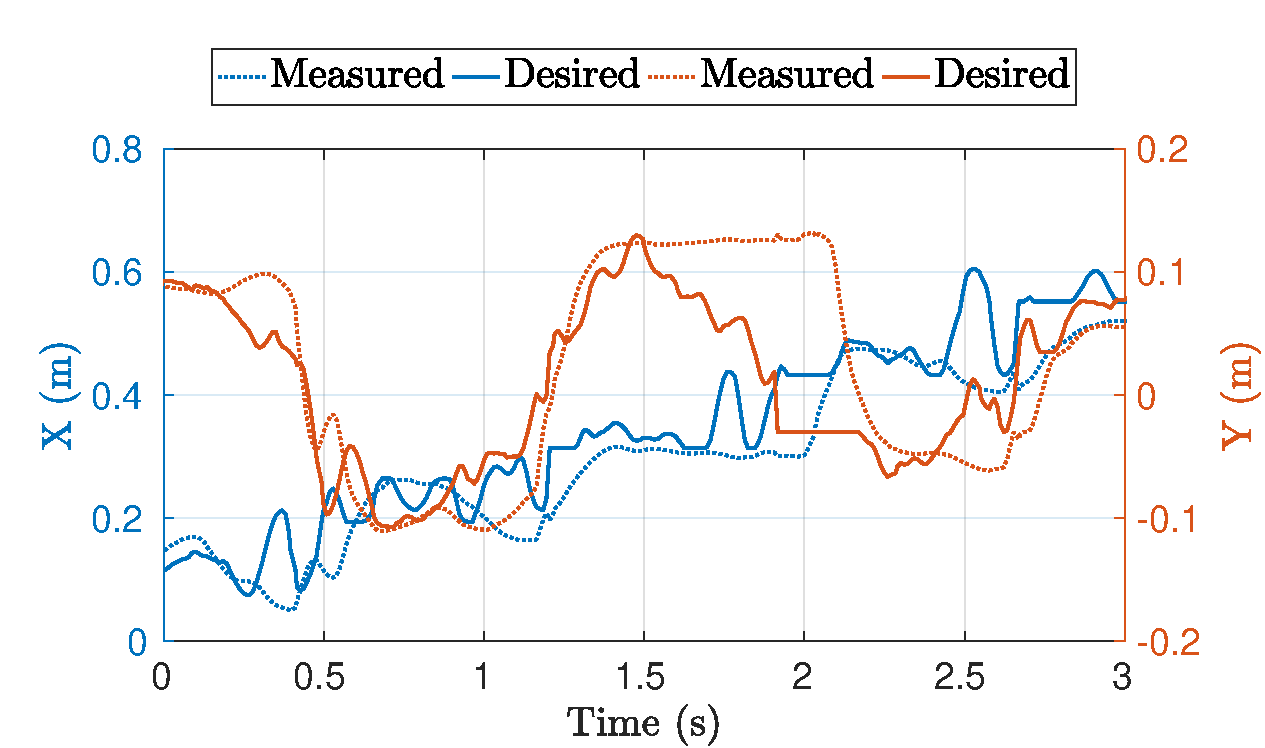
\includegraphics[width=\textwidth]{chapter_simplified_benchmarking/figures/mpc_pos-max_vel-zmp.pdf}
        \caption{ZMP}
        \label{fig:mpc_pos-max_vel-zmp}
    \end{subfigure}
    \end{myframe}
    \caption{Tracking of the  DCM (a), CoM (b) and ZMP (c) with the predictive and whole-body QP control as position control. At $t\approx \SI{2}{\second}$, the robot falls down.  Walking velocity: $\SI{0.41}{\meter \per \second}$.}
    \vskip-0.5cm
\end{figure}

We compare the control laws~\eqref{eq:reactive_dcm} and~\eqref{eq:mpc_solution_simplified}, which both generate a (desired) center of pressure that attempts to stabilize the desired DCM. To simplify the comparison, the controller of the \emph{whole-body QP layer} is kept fixed in this section, and we show and discuss only the results when the robot is position controlled. A complete comparison of the kinematics-based whole-body controllers is presented in Section~\ref{sec:wbc_experimental_results}.
In the following experiments, we set the time horizon of the predictive control to $\SI{2}{\second}$.

\subsection{Experiment 1: a forward robot speed of 0.1563 m s$^{\text{-1}}$}
Figures \ref{fig:inst_pos-min_vel-dcm} and \ref{fig:mpc_pos-min_vel-dcm} show the DCM tracking performances obtained with the instantaneous and predictive controllers, respectively. Both controllers seem to show good tracking performances, and the DCM error is kept below $\SI{5}{\centi \meter}$ in both cases. Note, however, that the instantaneous controller induces faster variations of the measured DCM. This contributes to the overall higher vibrations of the robot. One of the reasons for this variation is that the instantaneous controller~\eqref{eq:reactive_dcm} injects a (desired) center of pressure proportional to the measured DCM, which in turn contains the center of mass velocity. To mitigate this, we may filter the joint velocities appropriately. However, in our case, the joint velocities were not filtered to avoid delays in the measured DCM. Our experience showed that adding a filter to joint velocities is not an easy task, and we did not find the right trade-off for obtaining overall performance improvements. 

Figures~\ref{fig:inst_pos-min_vel-com} and \ref{fig:mpc_pos-min_vel-com} present CoM tracking performances, which are mainly dependent on the ZMP-CoM controller~\eqref{eq:ZMP_controller}. This controller receives the desired DCM values from the \emph{simplified model control} layer, which are obtained with the instantaneous or predictive controllers. In both cases, the CoM error is kept below $\SI{2}{\centi \meter}$. Figures~\ref{fig:inst_pos-min_vel-zmp} and~\ref{fig:mpc_pos-min_vel-zmp} represent the ZMP tracking performance, which is still mainly dependent on the ZMP-CoM controller~\eqref{eq:ZMP_controller}. It is important to note that the desired ZMP is smoother when the \emph{simplified model control} uses the predictive law~\eqref{eq:mpc_solution_simplified} to generate it. Indeed, this is a tunable property that depends on the associated weight in the cost function of the MPC problem. Although this smoother behavior contributes to less robot vibrations, overall robot performance became less reactive and, consequently, less robust to robot falls. Although the extensive hand-made tuning, we were not able to increase the robot velocity when the \emph{simplified model control} used the predictive law~\eqref{eq:mpc_solution_simplified}. 

\subsection{Experiment 2: a forward robot speed of 0.3372 m s$^{\text{-1}}$}
At a robot's desired walking speed of $\SI{0.3372}{\meter \per \second}$, there is initially no significant difference between the DCM tracking obtained with instantaneous and predictive control laws -- see Figures~\ref{fig:mpc_pos-max_vel-dcm} and~\ref{fig:inst_pos-max_vel-dcm} for $t < \SI{1.5}{\second}$. However, fast robot walking velocities require fast variations of the desired CoM and ZMP. This fast variation degrades the performance of the predictive controller around $t = \SI{1.5}{\second}$ -- see Figure~\ref{fig:mpc_pos-max_vel-zmp}. Clearly, these bad performances, in turn, induce poor tracking of the DCM shown in Figure~\ref{fig:mpc_pos-max_vel-dcm} at $t\approx \SI{2}{\second}$, and consequently the robot falls. At this point, one is tempted to increase the gain $K_\text{ZMP}$ of the controller~\eqref{eq:ZMP_controller}, which shall induce a better tracking of the ZMP. Unfortunately, this leads to higher robot oscillations induced by the noise on the estimated ZMP. And, as a consequence, the robot falls. 

We can conclude that the \emph{predictive simplified control} is much less robust than the \emph{instantaneous simplified control} with respect to ZMP tracking errors. Adding a low-pass filter to the ZMP measurement may improve the overall performance. However, in our case, adding filters led to slower system response and, consequently, to the robot falling.



\section{Conclusions\label{sec:centroidal_mpc_conclusion}}
This chapter discusses the development of an online centroidal momentum non-linear MPC for humanoid robots. 
The controller aims to generate feasible contact locations and wrenches for locomotion.
Different from state-of-the-art architectures based on simplified models (e.g. LIPM), the proposed controller can be used to perform highly dynamic movements, such as jumping and running. Furthermore, the contact location adjustment is considered in the centroidal dynamics stabilization problem, so it is not required to design an ad-hoc block for this feature. We validate the controller with a simulation of one-leg and two-leg systems performing jumping and running tasks, respectively. 
The centroidal MPC is also embedded in the three-layer position-based control architecture and tested on the humanoid robot iCub v3 -- see Section~\ref{sec:iCub3}. The proposed strategy prevents the robot from falling while walking and pushed with external forces up to $\SI{40}{\newton}$ for 1 second applied to the robot arm.
\par
In future work, we may extend the MPC to consider the contact timing adjustment, thus increasing the robustness properties against unpredictable external disturbances.
Another interesting research direction is to substitute the Euler integrator required to transcribe the optimal control problem into an MPC~\ref{sec:mpc_formulation} with a multi-rate sampling technique~\citep{Elobaid2020Sampled-dataPlanning,Elobaid2019OnSampling}. Considering a multi-rate sampling technique, it would be possible to reduce the prediction model's discretization error. To improve the time performance, we may consider applying the convex relaxation of the angular momentum dynamics~\citep{Ponton2018,Ponton2016AGeneration} in the controller prediction model. As a consequence, it would be possible to solve the non-linear optimization problem~\eqref{eq:mpc_centroidal_contact_optimization} by using a convex programming solver and thus increasing the MPC frequency.  
Finally, to improve the overall time performance, we plan to warm start the non-linear optimization problem with the result of a human-like trajectory planner~\citep{Viceconte2022ADHERENT:Robots}.